\documentclass{report}
\usepackage{settings}  % подклчючение настроек документа

% Подавить бесполезные предупреждения
\hbadness=10000

\begin{document}

%%%% Вставка необходимого титульника %%%%
%\thispagestyle{titlepage} % Для размещения Иркутск в нижнем колонтитуле
%\newpage
    \begin{center}
    \linespread{1}
		Министерство науки и высшего образования  Российской Федерации\\
федеральное государственное бюджетное образовательное учреждение\\
высшего образования\\
«Иркутский государственный университет»\\
(ФГБОУ ВО «ИГУ»)\\
Факультет бизнес-коммуникаций и информатики 
    \end{center}
\vspace{1cm}    
\hspace{8cm} 
\begin{minipage}{0.5\textwidth}
\linespread{1}

  \begin{flushleft}
	\small{
    Кафедра естественнонаучных дисциплин \\%\vspace{-2cm}
Допускается к защите \\
и.о. зав. кафедрой, к.ф.-м.н., доцент \\
\rule{2,1cm}{0,1pt} А.Г. Балахчи\\		
            «\rule{0,9cm}{0,1pt}»\rule{2,7cm}{0,1pt} 202\,\rule{0,2cm}{0,1pt} г \\		}
		%\vspace{2еm}
		
		
		%\vspace{4.0em}
		\end{flushleft}
\end{minipage}


    \vspace{2cm} %вертикальное расстояние
    \begin{center}
   {\bf ВЫПУСКНАЯ КВАЛИФИКАЦИОННАЯ РАБОТА БАКАЛАВРА ИЛИ КУРСОВАЯ РАБОТА\\
    по направлению  \\
		09.03.03 Прикладная информатика\\
		%\vspace{1em}
		профиль\\
		«Название профиля»\\}
    \end{center}
		
		%\vspace{2.5em}%вертикальное расстояние
    \begin{center}
  		Название выпускной квалификационной работы или курсовой работы\\
    \end{center}
		
		\vspace{2.5em}
		
   \hspace{-5em} 


\noindent
\begin{minipage}[t]{0.5\textwidth}
  \begin{flushleft}
  \linespread{1}
	\small{
    Консультант: должность, ученое звание \\
  Место работы\\
        \rule{1,8cm}{0,1pt} ФИО (в именительном падеже)\\
	\vspace{2em}
		
	Нормоконтролёр: должность, уч. зв,\\
            \rule{1,8cm}{0,1pt} ФИО (в им. падеже)\\
}
		%\vspace{2em}
		
		
		%\vspace{4.0em}
		\end{flushleft}
\end{minipage}%\hspace{1em} 
\begin{minipage}[t]{0.5\textwidth}
  \begin{flushleft}
  \linespread{1}
	\small{
    Студент ** курса
	** формы обучения \\
  группа **\\
        \rule{1,8cm}{0,1pt} ФИО (в им. падеже)\\
	\vspace{2em}
		
	Руководитель: уч. степень, уч. звание\\
            \rule{1,8cm}{0,1pt} ФИО (в им. падеже)\\
\vspace{2em}
 Работа защищена:\\
        «\rule{0,9cm}{0,1pt}»\rule{2,7cm}{0,1pt} 202\,\rule{0,2cm}{0,1pt} г \\
с оценкой \rule{1,8cm}{0,1pt}\\
Протокол № \rule{0,9cm}{0,1pt}}
		%\vspace{2em}
		
		
		%\vspace{4.0em}
		\end{flushleft}
\end{minipage}
\vfill

% Изменить год в надписи <<Иркутск 202*>> нужно в файле settings.sty на 221 строке

\newpage  % Титульный лист дипломной работы 
%\thispagestyle{titlepage}
%\newpage

    \begin{center}
    \linespread{1}
		Министерство науки и высшего образования  Российской Федерации\\
федеральное государственное бюджетное образовательное учреждение\\
высшего образования\\
«Иркутский государственный университет»\\
(ФГБОУ ВО «ИГУ»)\\
Факультет бизнес-коммуникаций и информатики 
    \end{center}
\vspace{1cm}    
\hspace{8cm} 
\begin{minipage}{0.5\textwidth}
\linespread{1}
%подписи для ВКР в курсовой можно удалить или заменить на настройку вертикального расстояния
  \begin{flushleft}
	\small{
    Кафедра естественнонаучных дисциплин \\%\vspace{-2cm}
Допускается к защите \\
и.о. зав. кафедрой, к.ф.-м.н., доцент \\
\rule{2,1cm}{0,1pt} А.Г. Балахчи\\		
            «\rule{0,9cm}{0,1pt}»\rule{2,7cm}{0,1pt} 202\,\rule{0,2cm}{0,1pt} г \\		}
		%\vspace{2еm}
		
		
		%\vspace{4.0em}
		\end{flushleft}
\end{minipage}


    \vspace{2cm} %вертикальное расстояние
    \begin{center}
   {\bf ВЫПУСКНАЯ КВАЛИФИКАЦИОННАЯ РАБОТА БАКАЛАВРА ИЛИ КУРСОВАЯ РАБОТА\\
    по направлению  \\
		09.03.03 Прикладная информатика\\
		%\vspace{1em}
		профиль\\
		«Название профиля»\\}
    \end{center}
		
		%\vspace{2.5em}%вертикальное расстояние
    \begin{center}
  		Название выпускной квалификационной работы или курсовой работы\\
    \end{center}
		
		\vspace{2.5em}
		
   \hspace{-5em} 


\noindent
\begin{minipage}[t]{0.5\textwidth}
  \begin{flushleft}
  \linespread{1}

		%\vspace{2em}
		
		
		%\vspace{4.0em}
		\end{flushleft}
\end{minipage}%\hspace{1em} 
\begin{minipage}[t]{0.5\textwidth}
  \begin{flushleft}
  \linespread{1}
	\small{
    Студент ** курса
	** формы обучения \\
  группа **\\
        \rule{1,8cm}{0,1pt} ФИО (в им. падеже)\\
	\vspace{2em}
		
	Руководитель: уч. степень, уч. звание\\
            \rule{1,8cm}{0,1pt} ФИО (в им. падеже)\\
\vspace{2em}
 Работа защищена:\\
        «\rule{0,9cm}{0,1pt}»\rule{2,7cm}{0,1pt} 202\,\rule{0,2cm}{0,1pt} г \\
с оценкой \rule{1,8cm}{0,1pt}\\
Протокол № \rule{0,9cm}{0,1pt}}
		%\vspace{2em}
		
		
		%\vspace{4.0em}
		\end{flushleft}
\end{minipage}

    \vfill
% Изменить год в надписи <<Иркутск 202*>> нужно в файле settings.sty на 221 строке
    
\newpage  % Титульный лист курсовой работы

\includepdf[pages={1}]{TitlePages/praktika.pdf} % Ваш титульний лист в .pdf 

%(если ваш титульный лист в формате .docx - воспользуйтесь сервисом по конвертации из docx (Word) в pdf)


\setcounter{page}{2} % начинаем нумерацию страниц
\tableofcontents  % это содержание, которое генерируется автоматически

\setcounter{chapter}{0} % установка счетчика глав
\setcounter{section}{0} % установка счетчика разделов
\setcounter{subsection}{0} % установка счетчика подразделов
\setcounter{equation}{0} % установка счетчика формул


\chapter*{ВВЕДЕНИЕ} % звездочка нужна, чтобы не было нумерации у этой главы
\addcontentsline{toc}{chapter}{ВВЕДЕНИЕ} % чтобы глава отображалась в содержании

В ИСЗФ СО РАН имеется уникальная научная установка --- Иркутский Радар Некогерентного Рассеяния (ИРНР). Всего в мире существует несколько подобных радаров, а ИРНР --- единственный в России. Данный инструмент является большой радиолокационной станцией, используемой для изучения процессов, происходящих в ионосфере Земли, а также для экспериментов по наблюдению за космическими объектами.

Радиолокационные станции являются сложными системами с большим количеством компонентов и разнятся по своей структуре. В общем случае, принцип действия радиолокационной станции заключается в излучении мощного зондирующего импульса и получении маломощного эхо, отразившегося от среды или объекта. В излучении участвует задающая часть, передатчики и антенна, совместно образующие передающий тракт --- набор компонентов, через которые проходит путь следования сигнала при излучении. Для приёма задействуется приёмный тракт, который состоит из антенны, усилителей, фильтров и регистрирующего комплекса.

Влияние приёмного и передающего тракта на проходящие через них сигналы прямым образом сказывается на способности радиолокационной станции получать достоверные данные в процессе наблюдений. В силу своей неидеальной природы, оборудование может искажать сигналы, ослаблять их и вносить задержки --- что очень критично в задачах с высокими требованиями к точности, например при определении расстояния до объекта на орбите на основе задержки радарного эхо.

В связи с этим возникает потребность в регулярной диагностике оборудования для оценки его характеристик (задержка, амплитудно-частотная характеристика, фазово-частотная характеристика и их стабильность) чтобы учесть их в дальнейшем на этапе обработки полученных данных.

Кроме того, высокочувствительное оборудование приёмного тракта может быть легко повреждено в силу своей близости к мощному излучению передатчиков, в связи с чем также возникает потребность в возможности быстрого обнаружения отказов приёмного тракта, что позволило бы обеспечить своевременное проведение ремонтных работ и помогло бы снизить общее время простоя.

Подобные потребности присущи не только ИРНР, но радиолокационным станциям в целом. Как правило, они решаются при помощи встроенных и тесно интегрированных средств диагностики, приспособленных под особенности строения конкретной станции. На текущий момент в составе ИРНР нет отдельной системы для диагностики, и задача измерения характеристик приёмного тракта решаются при помощи методов пассивной калибровки по излучению звёздных радиоисточников, что обладает ограниченной оперативностью, а обнаружение отказов происходит путём визуального осмотра получаемых в процессе наблюдений данных, что тоже обладает ограниченной оперативностью.

Для более тщательного решения данных задач в рамках ИРНР предлагается разработка узкоспециализированного программно-аппаратного комплекса для диагностики и исследования характеристик его приёмного тракта. В состав комплекса входит программируемый генератор тестовых сигналов, построенный на основе цифрового синтезатора сигналов AD9910 и микроконтроллера STM32 со встроенным ПО на языке программирования Си, а также пакет программных инструментов для управления и аналитики на языке программирования Python.

Принцип действия системы заключается в использовании программируемого генератора сигналов для подачи тестовых сигналов известной формы на вход приёмного тракта ИРНР и использовании штатного регистрирующего комплекса радара для получения записей сигналов. Затем, на основе анализа различий между полученным в действительности сигналом и прогнозировавшимся на основе модели сигналом выполняется оценка характеристик приёмного тракта.

Внедрение подобного решения на постоянной основе позволило бы регулярно выполнять активную калибровку приёмного тракта ИРНР и с высокой оперативностью проводить диагностику в случае возникновения подозрений на отказ оборудования. В дальнейшем, информация о характеристиках приёмного тракта может использоваться для повышения точности измерений в научных задачах.

{\bf Объект исследования:} приборостроение и автоматизация.

{\bf Предмет исследования:} программно-аппаратные комплексы и контрольно-измерительное оборудование.

{\bf Цель исследования:} создание программно-аппаратного комплекса, позволяющего расширить диагностические возможности ИРНР и предусматривающего возможность внедрения на постоянной основе.

{\bf Задачи:}
\begin{enumarabic}
\item расширение возможностей разработанного ранее программируемого генератора тестовых сигналов;
\item разработка гибкого форматов файлов конфигураций для описания диагностических сценариев;
\item разработка программных инструментов для проведения измерений и получения результатов в полуавтоматическом режиме.
\end{enumarabic}


{\bf Теоретическая новизна исследования} заключается в разработке приспособленных под особенности ИРНР подходов к проведению диагностических измерений, в разработке методов управления для применения цифрового синтезатора сигналов AD9910 в роли гибкого генератора тестовых сигналов, обладающего возможностями, которые обычно встречаются только в гораздо более дорогостоящих решениях. Также новизной обладают разработанные форматы данных, которые позволяют описывать сложные диагностические сценарии.

{\bf Практическая значимость исследования (если есть)} заключается в развитии диагностических возможностей ИРНР.

% 
\setcounter{section}{0} % обнуление счетчика разделов перед новой главой
\setcounter{subsection}{0} % обнуление счетчика подразделов перед новой главой
\setcounter{equation}{0} % обнуление счетчика формул перед новой главой

\chapter{ТЕОРЕТИЧЕСКИЕ ОСНОВЫ ДИАГНОСТИКИ РАДАРОВ}

\section{Обзор предметной области}

Архитектура каждой отдельно взятой радиолокационной станции зависит от специфики выполняемых задач, но в общем случае радиолокационные станции являются технологически сложными системами, сочетающими в себе высокие требования к мощности создаваемого излучения и высокие требования относительно чувствительности к получаемому излучению. Компоненты в составе РЛС подвержены воздействиям, которые редко встречаются где-либо ещё.

Время между излучением зондирующего импульса и получением отражённого сигнала часто составляет малые доли секунды, что также приводит к большим требованиям касательно синхронизации между передающим и приёмным оборудованием станции.

Работая в таких тяжёлых условиях, оборудование станции подвержено износу. Это может выражаться как в постепенной деградации отдельных компонентов, так и в неожиданных отказах. Также играет роль человеческий фактор --- возможно допущение ошибок, особенно во время обслуживания оборудования, что может заключаться, например, в неправильном подключении кабелей. Всё это может ухудшить качество получаемых данных или вообще воспрепятствовать проведению наблюдений.

В связи с этим радиолокационные станции обычно имеют в своём составе диагностические средства, которые призваны помочь в оценке состояния оборудования. Их набор может включать всё от измерительных устройств для проверки состояния отдельных элементов системы до генераторов тестовых сигналов, которые тестируют группы компонентов в сквозном режиме.

Приёмный тракт станции является одной из подсистем, которые целесообразно тестировать в сквозном режиме. Роль приёмного тракта заключается в усилении слабых сигналов полученных антенной и их преобразовании в вид, который пригоден для дальнейшей обработки в рамках регистрирующего комплекса. Приёмный тракт, в частности его отдельные каналы, обладают последовательным строением: подключенные друг за другом ключи, фильтры, усилители, и связующие их кабели. Характеристики приёмного тракта являются произведением характеристик всех его частей, и отказ одного элемента приведёт к неработоспособности всего тракта.

РЛС Днепр, которая лежит в основе ИРНР, предусматривала средства для тестирования приёмного тракта, однако они не сохранились после множества модернизаций и в любом случае были бы устаревшими по современным меркам. Данная работа посвящена разработке нового диагностического средства для сквозного тестирования приёмного тракта ИРНР.

С точки зрения пропускания сигналов, основными характеристиками  приёмного тракта (и его составляющий частей) можно считать амплитудно-частотную характеристику и фазо-частотную характеристику.

Амплитудно-частотная характеристика (АЧХ) определяется ослаблением или усилением, которое представлено выраженным от частоты коэффициентом. Усилением обладают, как правило, только усилители. Фильтры же ослабляют сигналы, причём таким образом, чтобы исключить нежелательные частоты и оставить только желаемые. Усиление приёмного тракта напрямую влияет на то, насколько слабые сигналы может обнаружить станция.

Фазо-частотная характеристика (ФЧХ) определяется смещением фазы между сигналом на входе и сигналом на выходе, в зависимости от частоты, что, в свою очередь, напрямую определяется задержкой, которую вносит устройство. Причём, одинаковая задержка вызовет более сильное смещение фазы для колебаний, которые выше по частоте. В связи с тем, что скорость распространения сигналов конечна, кабели любой длины будут обладать некоторой ФЧХ.

% TODO: доп. про почему важно усиление

Данные характеристики можно присвоить любым системам, которые работают с сигналами, в частности цифровым фильтрам. В цифровом представлении, несложно получить идеальное усиление или ослабление сигналов: достаточно умножить на выбранный коэффициент значения сигнала от времени, и результатом будет усиление или ослабление всех частот в сигнале. Похожим образом можно с абсолютной точностью измерить характеристики цифровых систем преобразования сигналов.

Реальный приёмный тракт, однако, состоит из реальных устройств, которые работают с токами высокой частоты (радиочастотных устройств). На высоких частотах паразитные ёмкости и паразитные индуктивности начинают играть большую роль и затрудняют измерения, в связи с чем измерение АЧХ и ФЧХ реальных устройств на высоких частотах считается сложной задачей, к которой нужно подходить с большой осторожностью.

% токи высокой частоты: нужен источник
% радиочастотные устройства: нужен источник
% считается сложной задачей: нужен источник

В контексте ИРНР, амплитудно-частотная характеристика и фазо-частотная характеристика приёмного тракта оказывают влияние на точность оценки пространственного положения источников сигнала в поле зрения антенны.

Антенна ИРНР является антенной с частотным сканированием, то есть это антенна, которая может электронно изменять направление луча, несмотря на своё фиксированное положение в пространстве. Во время излучения, отклонение луча вдоль большой оси антенны происходит при помощи изменения частоты сигнала. Во время приёма, антенна обладает зависящей от частоты чувствительностью для каждого возможного угла в поле зрения вдоль большой оси.

Можно представить ситуацию, когда в антенну ИРНР под некоторым углом вдоль большой оси приходит сигнал с равным содержанием всех частот; исходя из того, на какой частоте антенна воспримет больше всего мощности, можно установить угол. Однако, вследствие неравномерного усиления приёмного тракта, некоторая ложная частота может быть воспринята как частота с максимальной мощностью, что помешает точной оценке угла. В связи с этим желательно знать и учитывать амплитудно-частотную характеристику приёмного тракта.

Другим методом происходит определение угла вдоль малой оси антенны. Внутренне антенна при помощи перегородки разделена на два полурупора, которые образуют два канала приёма. Когда сигнал достигает антенны под некоторым углом вдоль малой оси, он достигнет дальний полурупор с некоторой задержкой относительно ближнего полурупора, что приведёт к возникновению разности фаз между полурупорами и соответствующими им каналами, причём разность пропорциональна углу. Таким образом, определив разность фаз можно определить угол. Однако, два канала приёмного тракта вносят собственную задержку в сигнал, и если задержка между ними различается, то наблюдаемая на выходе разность фаз изменится от исходной, что также помешает точной оценке угла. На высоких частотах, небольшие различия в длине кабелей и производственный разброс характеристик между номинально одинаковыми компонентами могут создавать различия между внешне одинаковыми по строению каналами приёмного тракта. В связи с этим желательно знать и учитывать фазо-частотную характеристику приёмного тракта.

Представленные ранее проблемы решаются методами пассивной калибровки по излучению космических радиоисточников, которые позволяют установить соответствие между достоверно известным положением объектов на небе и тем, что воспринимает оборудование станции. Это не отменяет потребности в системе диагностики для приёмного тракта; наличие средства для активной калибровки стало бы хорошим дополнением к методам пассивной калибровки.

Из этого исходят два основных сценария использования диагностической системы в рамках ИРНР:

\begin{enummarker}
    \item оценка АЧХ;
    \item оценка ФЧХ (в частности разности фаз между каналами).
\end{enummarker}

% https://planarchel.ru/instruction/rvna/principle-of-measuring-s-param.html

Широко используемым инструментом для оценки АЧХ и ФЧХ являются векторные анализаторы цепей (VNA), которые представляют собой готовое решение специально предназначенное для выполнения данной задачи. Чаще всего они существуют в форме автономного устройства, но встречаются также варианты, подключаемые к компьютеру.

Принцип действия VNA заключается в подаче сигнала на вход тестируемого устройства и измерении, одновременно, комплексных амплитуд (амплитуды и фазы) падающего сигнала, отраженного сигнала, и прошедшего через исследуемое устройство сигнала. На основе отношения комплексных амплитуд вычисляются так называемые S-параметры, которые описывают АЧХ и ФЧХ исследуемого устройства. Данное измерение происходит на множестве частот в цикличном режиме, и программное обеспечение VNA предусматривает возможность усреднения по пройденным несколько раз точкам, чтобы исключить влияние шума.

Многие векторные анализаторы цепей используют непрерывный сигнал, но существуют также импульсные VNA, которые могут подавать короткие импульсы по внешнему синхронизационному сигналу. Импульсный режим встречается только на более дорогих устройствах, но необходим в сценарии с использованием на ИРНР в связи с одной уникальной особенностью окружающей среды --- поблизости расположена другая радиолокационная станция, работа передатчиков которой создаёт мощные помехи для работы любого измерительного оборудования, не интегрированного со специальной системой синхронизации между двумя станциями.

Кроме того, вне зависимости от стоимости, набор функций в готовых VNA фиксирован и не предполагает возможности расширения, а сопутствующее ПО не имеет открытого исходного кода, что сильно ограничивает возможности по взаимодействию с другим ПО в целях автоматизации.

В связи с высокой стоимостью подобных устройств, а также обозначенными выше недостатками, внедрение VNA в роли диагностического средства для приёмного тракта ИРНР не рассматривается.

% План по содержанию:
% ЧАСТЬ 1. ОБЗОР ПРЕДМЕТНОЙ ОБЛАСТИ
% - Задачи диагностики радаров
%     - История
%         - Конечно
%     - Возможности
%         - Группы тестов
% - Характеристики РЧ устройств
% - Специфика измерений на ИРНР
%     - Характеристики ИРНР
%     - Затухание
%     - Разность фаз между каналами
% - Векторные анализаторы спектра
%     - Трудности
% - Векторные генераторы сигналов
%     - Дорогие
%     - В итоге сделали свой

% ЧАСТЬ 2. АЛГОРИТМЫ

% - Регистрирующий комплекс даёт IQ
% - Мы делаем графики из IQ

Первая глава чаще носит теоретический характер. Прописываются инструменты, которые используются в работе, обсуждается сравнение нескольких инструментов и обосновывается, почему был сделан выбор в пользу определенных инструментов. Делается анализ литературы по теме курсовой работы: кто еще делал подобные исследования и какие были результаты, как вообще проводятся исследования задач, подобных задачам в курсовой, какие подходы существуют, и почему был выбран именно такой подход.

\section{Общие нюансы оформления работы с использованием шаблона \LaTeX}
Курсовая или дипломная работа оформляется по требованиям ИГУ основанных на ГОСТ 7.32---2001 с некоторыми изменениями. То, что там не прописано можно брать из более свежего ГОСТ 7.32---2017 <<Отчёт о научно-исследовательской работе>>. Шаблон оформлен в соответствии с этим требованиями ИГУ и ГОСТ 7.32---2017. 

Важные советы будут прописаны как в тексте шаблона, так и в комментариях к коду. Более подробная информация находится в методических материалах к этому шаблону.

Список использованных источников должен быть выполнен в соответствии с ГОСТ Р ГОСТ 7.1—--2003 <<Библиографическая запись. Библиографическое описание. Общие требования и правила составления>>. Несколько примеров оформления источников будут представлены в соответствующей главе.

Максимальная вложенность подглав в курсовой или дипломной работе --- 2 уровень. То есть, подглавы 1.1.1 в курсовой работе быть не может. Если необходим такой уровень, то пишется название на новой строке с красной строки без точки на конце, выделять жирным не нужно. Пример ниже.

Пример заголовка третьего уровня

Если вы описываете своими словами или напрямую цитируете текст другой работы, то нужно указать такую метку \cite{bib_gost1}. В тексте работы должны находиться ссылки на все источники из списка использованных источников. Если вы хотите сослаться сразу на несколько работ, то метка выглядит так \cite{bib_gost2}---\cite{bib_electr_res}. Источники в списке должны идти в том порядке, в котором они упоминаются в тексте. Проверяйте, что ссылки сработали правильно, и там не стоят знаки вопроса [?].

Следите за использованием тире (---) и дефисов (-). Дефис — орфографический знак, разделяющий части слова (всё-таки, во-первых), короткий, без пробелов.
Тире — пунктуационный знак, ставится между словами, длинное, отделяется пробелами с обеих сторон. Пример использования тире: Грамоте учиться — всегда пригодится. Пример использования дефиса: Разрабатывая веб-приложение, программист сталкивается с необходимостью оптимизации базы данных.

Обращайте внимание на переносы строк в тексте вашей работы. Бывает, что получаются <<висячие строки>> (когда меньше 3 букв на строке), которых не должно быть в работе. Пример изображен на рисунке \ref{fig:pic11}. В таких ситуациях следует вручную указать перенос строки с помощью \verb|\break|. Так же помните про правила переноса тире.

% Классический способ вставки рисунка
% \vspace{3mm}
% \begin{figure}[h]
% \centering
%     
\includegraphics[width=0.9\linewidth]{vis_str.png}
%     \captionsetup{justification=centering, format=plain}
%     \caption{Висячая строка}
%     \label{fig:pic11}
% \end{figure}

% Краткий способ вставки рисунка
\myfigure{0.9}{vis_str.png}{Висячая строка}{pic11}

Не допускайте разделения на две страницы названия раздела и текста раздела, списка, рисунка и подписи к рисунку, таблицы и подписи к таблице. В таких случаях можно использовать тот же \verb|\break|, комбинацию команд \verb|\hfill\break| для смещения на одну строку или команду \verb|\newpage|, которая переносит последующий текст на следующую страницу.


Крайне важно следить за орфографией и пунктуацией текста вашей работы. \LaTeX\ будет контролировать правописание, если в левом верхнем углу в Menu(Меню) --> Spell check (Проверка орфографии) поставить русский язык, но намного удобнее воспользоваться сторонним инструментом. Для проверки орфографии, пунктуации и стилистики вашего текста существует расширение для браузера Chrome под названием LanguageTool (https://languagetool.org/ru/overleaf), которое совместимо с Overleaf. Кроме того, данное расширение предлагает и другие полезные функции для работы с текстом.

\section*{Выводы по главе}
\addcontentsline{toc}{section}{Выводы по главе}
В данной главе было рассмотрено ... (Краткое обобщенное описание того, что было в главе).


\chapter{НАЗВАНИЕ ВТОРОЙ ГЛАВЫ КУРСОВОЙ ИЛИ ВЫПУСКНОЙ КВАЛИФИКАЦИОННОЙ РАБОТЫ}
% снова обнуляем счетчики section, subsection и equation в новой главе
\setcounter{section}{0}
\setcounter{subsection}{0}
\setcounter{equation}{0}
\section{Название первого параграфа второй главы}

Вторая глава носит практическую направленность. В ней нужно описать процесс работы над темой. Подробно расскажите о том, как реализовано и устроено то, что вы сделали. Активно используйте небольшие рисунки, таблицы, формулы, листинги кода. 

\section{Оформление различных элементов}

Важно проследить за оформлением списков (перечислений) в своей работе. Перечисления бывают простые и сложные, маркированные и нумерованные. Перечисления отделяются точкой с запятой. В конце перечисления всегда точка. После цифры или буквы в нумерованном списке должна стоять только круглая закрывающаяся скобка. Буквы можно использовать строчные русского алфавита (за исключением букв ё, з, й, о, ч, ъ, ы, ь).
В этом шаблоне можно использовать кастомные списки: \verb|\begin{enummarker}| --- для маркированных списков, \break \verb|\begin{enumarabic}| --- для нумерованных списков, \verb|\begin{enumasbuk}| --- для нумерованный списков с русскими строчными буквами.

Пример 1

Что перепроверить перед сдачей работы нормоконтролеру:
\begin{enummarker}
\item заполнение титульного листа;
\item использование тире (---) и дефисов (-) в тексте;
\item переносы слов не выходят за правую рамку документа. 
\end{enummarker}

Пример 2

Что ещё перепроверить перед сдачей работы:
\begin{enumarabic}
  \item ссылка на рисунок, таблицу или формулу находиться до рисунка, таблицы или формулы;
  \item наличие ссылки на каждый рисунок, приложение и литературный источник в тексте работы;
  \item оформление списков, рисунков, таблиц и формул.
\end{enumarabic}

\hfill\break % чтобы не разрывать пример 3
\hfill\break
\hfill\break

Пример 3

Перечисление с русскими строчными буквами:
\begin{enumasbuk}
  \item первый элемент;
  \item второй элемент;
  \item третий элемент.
\end{enumasbuk}

Пример 4

Сложный список:

\begin{enummarker}
  \item в машиностроении:
    \begin{enumarabic}
        \item для очистки отливок от формовочной смеси;
        \item для очистки лопаток турбин авиационных двигателей;   
    \end{enumarabic}
  \item в ремонте техники:
    \begin{enumarabic}
        \item для очистки отливок от формовочной смеси;
        \item для очистки лопаток турбин авиационных двигателей.  
    \end{enumarabic}
\end{enummarker}


В больших списках,  особенно, где каждый пункт содержит несколько 
предложений, надо предварять список предложением с точкой, а не двоеточием, и далее все пункты заканчиваются точками. Важно сформулировать предложение, предваряющее список, как самостоятельное. Например, в мобильное приложение можно добавить следующие возможности. 
\begin{enummarker}
\item Первая возможность. Что-то о первой возможности.
\item Вторая возможность. Что-то о второй возможности.
\item Третья возможность. Что-то о третьей возможности.
\end{enummarker}


Вставка рисунка

Рисунки должны находится в папке Images. Путь к рисунку прописывается в \verb|\includegraphics|  в виде \{filename.png\}. Размер рисунка можно изменять с помощью параметра width. Название рисунка задаётся в параметре \verb|\caption|. На все рисунки должны быть ссылки. Рисунок должен идти непосредственно после ссылки или на следующей странице (как можно ближе). Ссылаться на номер рисунка можно по имени обозначенном в \verb|\label|. Пример: Существуют определенные правила использования кавычек в исследовательской работе (рис. \ref{fig:pic21}) \break или (см. рис. \ref{fig:pic21}). Ещё можно воспользоваться кастомизированной командой с 4 аргументами \verb|\myfigure{ширина}{имя файла}{подпись}{ссылка на рисунок}|. Примеры ее применения есть в коде.

% \begin{figure}[H]
% \centering
%     % width - отвечает за размер вашего рисунка
%     % {kavichki.png} - это название рисунка из папки Images
%     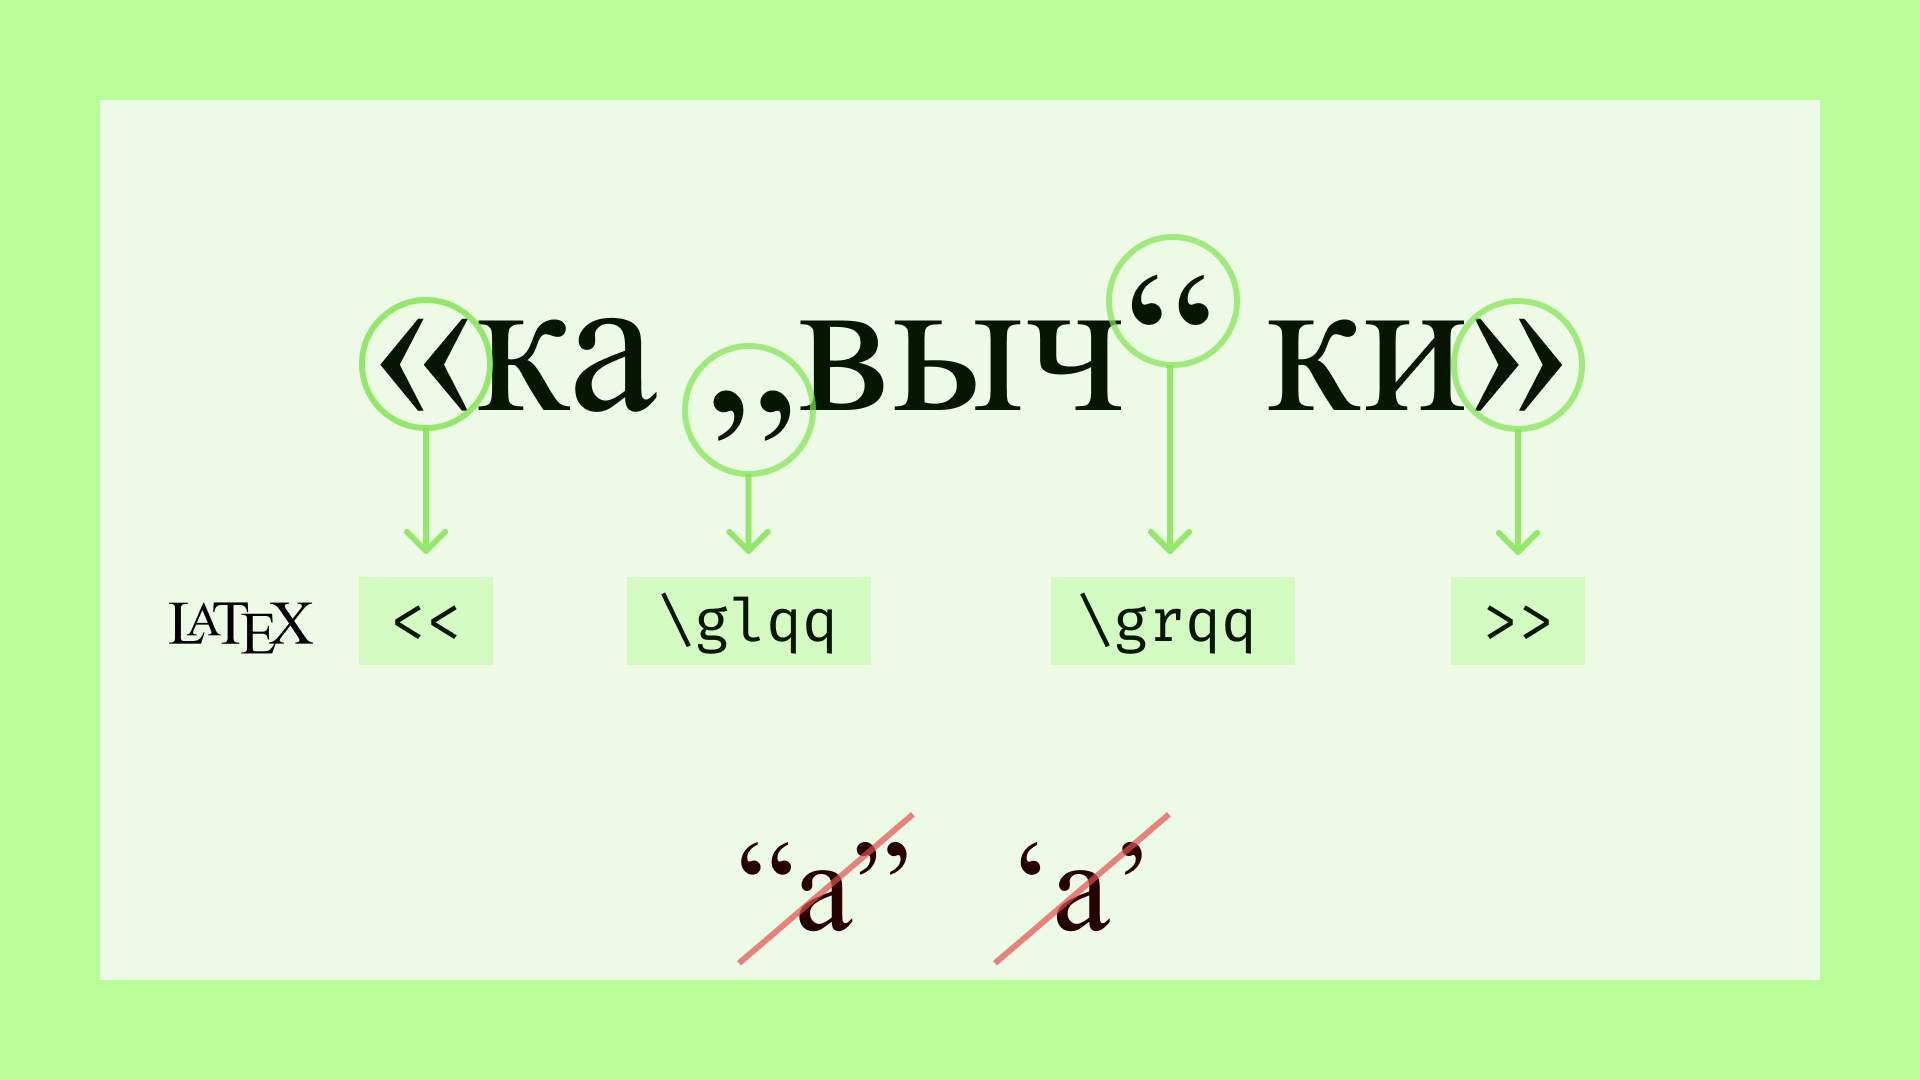
\includegraphics[width=0.9\linewidth]{kavichki.png}
%     \captionsetup{justification=centering, format=plain}
%     \caption{Правильное использование кавычек} % Название рисунка
%     \label{fig:pic21}
% \end{figure}

\myfigure{0.9}{kavichki.png}{Правильное использование кавычек}{pic21}

Вставка нумерованной формулы.
\begin{equation}
P_{gen}=P_{f} + P_S + P_C + P^3 + P_P
\label{eq}
\end{equation}

Вставка формулы в тексте \(P_{gen}=P_{f} + P_S + P_C + P_3 + P_P\). Рекомендуется использовать \verb|\[...\]| для выключенных (на отдельной строке) формул вместо \verb|$$...$$|.  Для встроенных в текст формул использовать  \verb|\(...\)|, а не \verb|$...$|. Ссылка на формулу --- формула (\ref{eq}).

Вставка таблиц

На все таблицы в тексте должны быть ссылки. Таблица должна располагаться непосредственно после текста, в котором она упоминается впервые, или на следующей странице. Пример ссылки на таблицу: Полученные данные занесены в таблицу \ref{table:table21}.

\renewcommand{\arraystretch}{2}  % увеличение высоты ячеек в 2 раза
\newcolumntype{C}{ >{\centering\arraybackslash} m{5cm} }  % создаем новый тип столбца с вертикальным центрированием (m), чтобы не дублировать длинную запись (указать нужную ширину в сантиметрах)
\begin{table}[h]
    \centering   % располагаем таблицу по центру
    \caption{Пример названия таблицы}    % название таблицы
    \begin{tabular}{|m{5cm}|C|C|}        % описываем 3 столбца таблицы
    \hline   % горизонтальная черта
    &  Заголовок столбца 1 & Заголовок столбца 2 \\ \hline
    Заголовок строки 1 & Значение & Значение \\ \hline
    Заголовок строки 2 & Значение & Значение \\ \hline
    \end{tabular}
    \label{table:table21}
\end{table}

Вставка длинной таблицы

Лучше избегать вставки длинной таблицы в тексте работы и перенести ее в приложение. 

Если это все-таки необходимо, важно не забывать писать <<Продолжение Таблицы (номер таблицы)>> или <<Окончание таблицы  (номер таблицы)>>, когда она переходит на новую страницу. Не нужно проводить черную линию перед переносом таблицы. Как это делать --- смотрите в коде документа. 

Если в вашей таблице числовые значения, то они хорошо смотрятся по центру ячейки, и тогда удобно создать новый тип столбца с нужными настройками, как сделано в первой маленькой таблице с помощью \verb|\newcolumntype|. Если в ячейках вашей таблицы находится текст, расположение по центру ему не всегда подходит. В таких случаях необходимо убрать центрирование в настройке столбца и вручную центрировать нужные ячейки с помощью \verb|\begin{center}| и \verb|\end{center}| или \verb|\centering|.

\hfill\break 
\hfill\break 
(пустое пространство, чтобы показать перенос таблицы)
\hfill\break 
\hfill\break 

\newcolumntype{J}{ >{\centering\arraybackslash} m{2cm} }
\newcolumntype{B}{ >{\centering\arraybackslash} m{6cm} } % здесь можно указать правило выравнивания и ширину стобца
% Из-за того, что мы прописали \centering в настройках столбцов выше, иногда нам придется использовать "\tabularnewline" вместо "\\"
\begin{longtable}[h!]{|J|B|B|}
    \caption{Название длинной таблицы} \\
    \hline
    № & Заголовок столбца 1 & Заголовок столбца 2 \tabularnewline
    \hline
    1 & 2 &  3 \tabularnewline
    \hline
    \endfirsthead
    \multicolumn{3}{r}{Окончание таблицы \thetable\hspace{-2em} } \tabularnewline  % корректируйте значение в \hspace{}, чтобы выровнять по правому краю

    \hline
     1 &  2 &  3 \tabularnewline 
    \hline
    \endhead

    \multicolumn{3}{l}{} 
    \endfoot

    \hline
    \endlastfoot


1 & Данные & Данные \\ \hline

2 & Данные & Данные \\ \hline

3 & Данные & Данные \\ \hline

4 & Данные & Данные \\ \hline

5 & Данные & Данные \\  \hline 

6 & Данные & Данные \\ \hline % на месте где разрывается таблица линию не проводим

7 & Данные & Данные \\ 

\end{longtable}

Листинг кода

Небольшой программный код, который нужно продемонстрировать в работе, можно представить в виде иллюстрации (скриншота) в тексте работы с соблюдением правил оформления для рисунков. В случае длинного листинга рекомендуется располагать его в приложении или иллюстрацией, или текстом. Пример оформления листинга в текстовом виде приведён в приложении Б. Вставка кода из файла продемонстрирована в приложении~В.



\section*{Выводы по главе}
\addcontentsline{toc}{section}{Выводы по главе}
Краткое описание того, что было в главе. Сделайте акцент на том, что было сделано вами лично.

\chapter*{ЗАКЛЮЧЕНИЕ}
\addcontentsline{toc}{chapter}{ЗАКЛЮЧЕНИЕ} % это будет отображаться в содержании

В заключении указывается основной результат работы и побочные результаты, если студент считает это необходимым. Дается оценка полноты решений поставленных задач. Прописывается, что планируется сделать в дальнейшем, если курсовая будет продолжаться в дипломе. 

Курсовая или дипломная работа подается на нормоконтроль за нес\-колько дней до защиты. Нормоконтролеру нужно высылать только pdf-файл, а после получения ответа от нормоконтролера ошибки устраняются, и работа посылается на проверку еще раз, и так до тех пор, пока нормоконтролер не одобрит работу.




\chapter*{СПИСОК ИСПОЛЬЗОВАННЫХ ИСТОЧНИКОВ}
\addcontentsline{toc}{chapter}{СПИСОК ИСПОЛЬЗОВАННЫХ ИСТОЧНИКОВ} % это будет отображаться в содержании
%\renewcommand{\bibsection}{\centering\textbf{\large СПИСОК ИСПОЛЬЗОВАННЫХ ИСТОЧНИКОВ}} % смена названия библиографии по умолчанию
%\bibliographystyle{biblio/gost2008n} % файл, задающий формат ссылок по ГОСТ
%\bibliography{biblio/biblio} % файл с библиографией

\begin{thebibliography}{}

\bibitem{bib_gost1}
    Отчёт о научно-исследовательской работе. Структура и правила оформления. : ГОСТ 7.32--2017 : национальный стандарт : дата введения 2018–07–01
    
\bibitem{bib_gost2} 
    Библиографическая запись. Библиографическое описание. Общие требования и правила составления : ГОСТ Р 7.0.100-–2018 : национальный стандарт : дата введения 2019-07–01
\bibitem{bib_electr_res} 
    Overleaf. Изучите LaTeX за 30 минут : [Электронный ресурс]. --– URL: https://www.overleaf.com/learn/latex/Learn\_LaTeX\_in\_30\_minutes \break(дата обращения: 21.03.2024).

\bibitem{bib_author}
    Вятчина О. Ф. Малый практикум по микробиологии : Учеб.-метод. пособие / О. Ф. Вятчина, Н. Е. Буковская, О. А. Жилкина. –- Иркутск : Изд-во Иркут. гос. ун-та, 2009. –- 129 с. : ил. –- Библиогр.: с. 128–129.

\bibitem{bib_setev_elect_res}
    Об объектах культурного наследия (памятники истории и культуры) народов Российской Федерации в Иркутской области [Электронный ресурс]  : закон Иркут. обл. от 23.07.2008 № 57-оз (в ред. От 05.042010). --– Документ опубликован не был. --– Доступ из справ. Правовой системы «КонсультантПлюс» в локальной сети Науч. б-ки Иркут. гос. ун-та.
    
\bibitem{bib_udal_res_site}
    Аргучинцев А. В. Оптимальное управление начальными условиями канонической гиперболической системы первого порядка на основе нестандартных формул приращения [Электронный ресурс] / А. В. Аргучинцев, В. П. Поплевко // Изв. вузов. Математика. –- 2008. --– № 1. --– С. 3–-10. --– Электрон. Версия печат. \breakПублик. . –- Систем. Требования: Adode Acrobat Reader/ --- URL: http: //ellib.librery.isu.ru/docs/social/p1422\_D19\_7525.pdf/ (дата обращения: 10.08.2010).

\end{thebibliography}


\chapter*{ПРИЛОЖЕНИЯ}
\addcontentsline{toc}{chapter}{ПРИЛОЖЕНИЯ}

% ДЛЯ ОТЧЕТОВ ПО ПРАКТИКЕ: вставить ежедневные записи студента можно по аналогии с титульном листом, таким образом:
% \addcontentsline{toc}{section}{Приложение А Ежедневные записи студента по практике}
% \includepdf[pages={1}]{vashi_zapisi_studenta.pdf} % файл конвертированный из docx с таблицей и всеми заголовками + номер страницы(!)

\begin{flushright}
     Приложение А
\end{flushright}

\begin{center}  Название приложения \end{center}
\addcontentsline{toc}{section}{Приложение А Название приложения}

Приложения обозначают заглавными буквами русского алфавита, начиная с А, за исключением букв Ё, З, Й, О, Ч, Ь, Ы, Ъ. После слова «Приложение» следует буква, обозначающая его последовательность.
Если в документе одно приложение, оно обозначается «Приложение А».
Каждое приложение начинается с новой страницы.
{\bf В тексте документа должны быть ссылки на все приложения.}  Приложения располагают в порядке ссылок на них в тексте документа.

Приложения могут включать: графический материал, таблицы, расчеты, описания алгоритмов и программ. Длинные таблицы, большие расчеты, длинные алгоритмы и программы рекомендуется помещать именно в приложения, а не в основной части работы. Здесь можно разместить ссылку на Github со своей работой, если нужно. Например, вот так:

Ссылка на репозиторий проекта: https://github.com/latex3/latex2e

Иллюстрации, таблицы, формулы в пределах каждого приложения обозначают отдельной нумерацией арабскими цифрами с добавлением впереди обозначения приложения (например: Рисунок А.1 или Таблица Б.2, к формуле просто (В.1)).
\newpage

\begin{flushright}
     Приложение Б
\end{flushright}

\begin{center}  Пример листинга кода \end{center}
\addcontentsline{toc}{section}{Приложение Б Пример листинга кода}

%% пропишите нужный вам язык программирования в language 
%% если рамка вокруг листинга вам не нужна - удалите параметр frame
\begin{lstlisting}[language=C, frame=single]  
#include <stdio.h>

int main() {
    int n, i, flag = 0;
    
    printf("Введите положительное целое число: ");
    scanf("%d", &n);
    
    for (i = 2; i <= n / 2; ++i) {
        // Проверка на простое число
        if (n % i == 0) {
            flag = 1;
            break;
        }
    }
    
    if (n == 1) {
        printf("1 не является ни простым, ни составным.\n");
    } else {
        if (flag == 0)
            printf("%d - простое число.\n", n);
        else
            printf("%d - составное число.\n", n);
    }
    
    return 0;
\end{lstlisting}
\newpage


\begin{flushright}
     Приложение В
\end{flushright}

\begin{center}  Второй пример листинга кода \end{center}
\addcontentsline{toc}{section}{Приложение В Второй пример листинга кода}

\lstinputlisting[language=python, frame=single]{Listings/main.py}


\newpage


\begin{flushright}
     Приложение Г
\end{flushright}

\begin{center}  Пример вставки рисунка \end{center}
\addcontentsline{toc}{section}{Приложение В Пример вставки рисунка}

В приложении лучше использовать классический способ вставки рисунка, где можно закомментировать подпись и ссылку, так как они нам здесь не нужны.

\begin{figure}[H]
\centering
    % width - отвечает за размер вашего рисунка
    % {kavichki.png} - это название рисунка из папки Images
    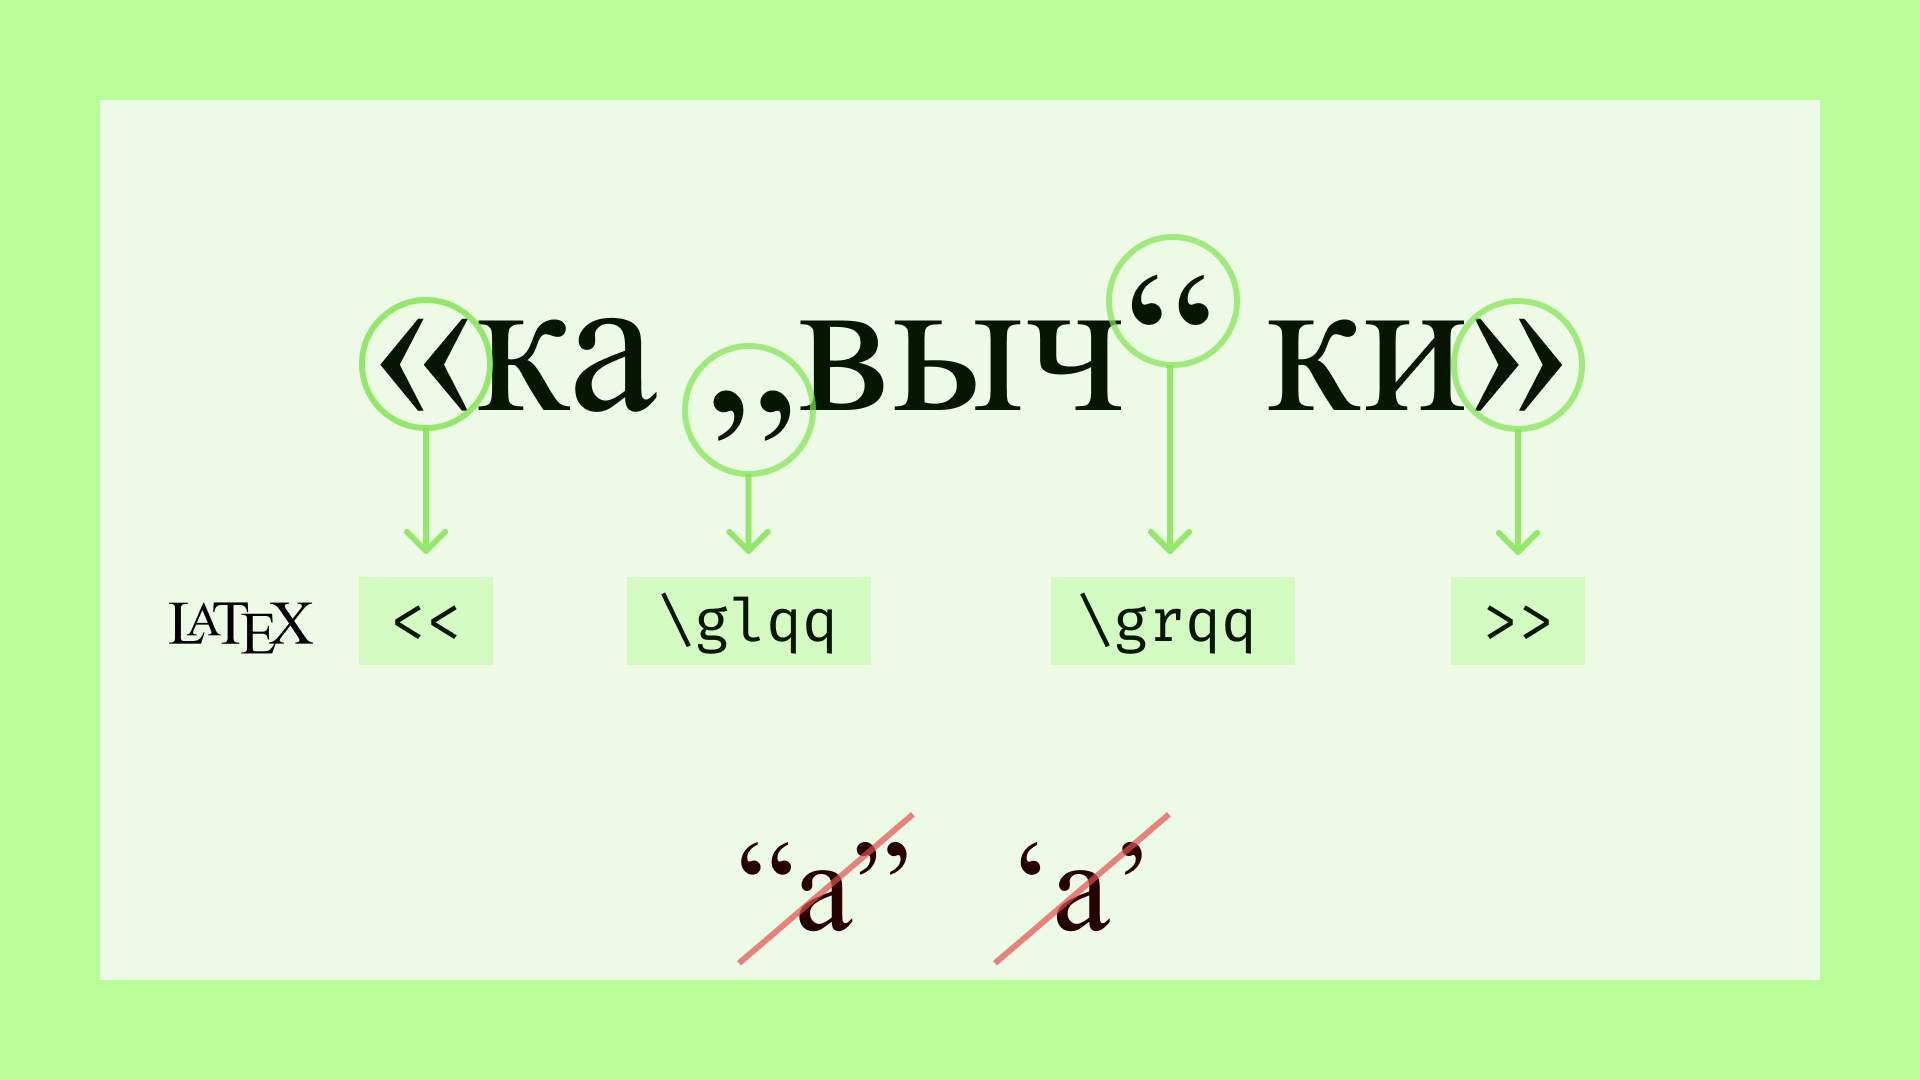
\includegraphics[width=1\linewidth]{kavichki.png}
    \captionsetup{justification=centering, format=plain}
    \caption{Правильное использование кавычек} % Название рисунка
    \label{fig:pic21}
\end{figure}

\end{document}

